\chapter{Background}
\label{background}

The chapter \textit{\nameref{background}} consists of the four sections \textit{\nameref{definition}}, \textit{\nameref{relatedsystems}}, \textit{\nameref{cliniscale}} and \textit{\nameref{relatedwork}}. The first section, \textit{\nameref{definition}}, explains basic terms to understand the topic of this thesis. The second section, \textit{\nameref{relatedsystems}}, presents an application similar to the CliniScale project. The third section, \textit{\nameref{cliniscale}}, presents the project this thesis is part of. The fourth section, \textit{\nameref{relatedwork}}, analyzes the current scientific landscape related to this thesis.


\section{Definitions}
\label{definition}
This section defines technical terms needed to understand this thesis.

\label{ciatriad}
\paragraph{CIA-Triad} A security model for the development of security policies within an organization, originally consisting of confidentiality, integrity and availability. The CIA-Triad is extended by three additional security properties: accountability, authorization and authenticity. 
\textbf{Confidentiality} is part of privacy. It describes the property that information is not made available or disclosed to unauthorized individuals, entities or processes. 
\textbf{Integrity} describes the property of maintaining consistency, accuracy and trustworthiness of data. 
\textbf{Availability} describes the property that authorized parties are able to access resources when needed. 
\textbf{Accountability} describes the security property of non-repudiation of every party to their actions. It prevents a party of denying performing an action, such as receiving or sending a transaction. 
\textbf{Authorization} defines the property defining if a party is allowed to access a resource after authentication. 
\textbf{Authenticity} describes the property of proper verification of a party's identity.


\paragraph{\textbf{General Data Protection Regulation (GDPR)}} The General Data Protection Regulation is a regulation in European Union (EU) law on data protection and privacy for all individuals within the EU and the European Economic Area implemented May 25, 2018\cite{GDPR}. The aim of the GDPR is to protect all EU citizens from privacy and data breaches. 


\paragraph{\textbf{Sensitive Personal Data}} Personal data which are by their nature particularly sensitive in relation to fundamental rights and freedoms are defined as sensitive personal data\cite{GDPR9}. They merit specific protection as the context of their processing could create significant risks to fundamental rights.

\paragraph{\textbf{Modular Risk Assessment (MoRA)}} The MoRA methodology is a security risk assessment methodology\cite{mora}. MoRA offers a risk-driven, iterative and modular approach and offers guidance and catalogs for practical application. The method is defined in chapter \ref{morachapter}.

\paragraph{Microsoft Threat Modeling Tool}\cite{mtmt} The Microsoft Threat Modeling Tool is a core element of the Microsoft Security Development Lifecycle. The tool allows software architects to identify and mitigate security issues early in the process of designing a software architecture. 
It is based on data flow diagrams to model the architecture. Threats get identified using the STRIDE threat classification scheme. The tool also consists of a security control catalogue, offering information on how to mitigate found threats.

\paragraph{Microsoft STRIDE} STRIDE is a threat model developed by Praerit Garg and Loren Kohnfelder at Microsoft\cite{stride}. The model helps identifying possible threats by categorizing them in six categories: Spoofing, Tampering, Repudiation, Information disclosure, Denial of service and Elevation of privileges.

\paragraph{Yakindu Security Analyst}\footnote{Yakindu Security Analyst: \url{https://www.itemis.com/en/yakindu/security-analyst/}. (Online; last accessed:  November 18, 2019)} The Yakindu Security analyst is a tool created by Itemis AG\footnote{Itemis AG: \url{https://www.itemis.com/en/}. (Online; last accessed:  November 18, 2019)} to perform risk assessments. It offers a highly customizable environment making it usable for different risk assessment methodologies. 


\section{Related System}
\label{relatedsystems}
\label{vivy}
This section presents a comparable application to the CliniScale system that exchanges sensitive personal data in a client server infrastructure using a mobile application.


\begin{figure}[H]
  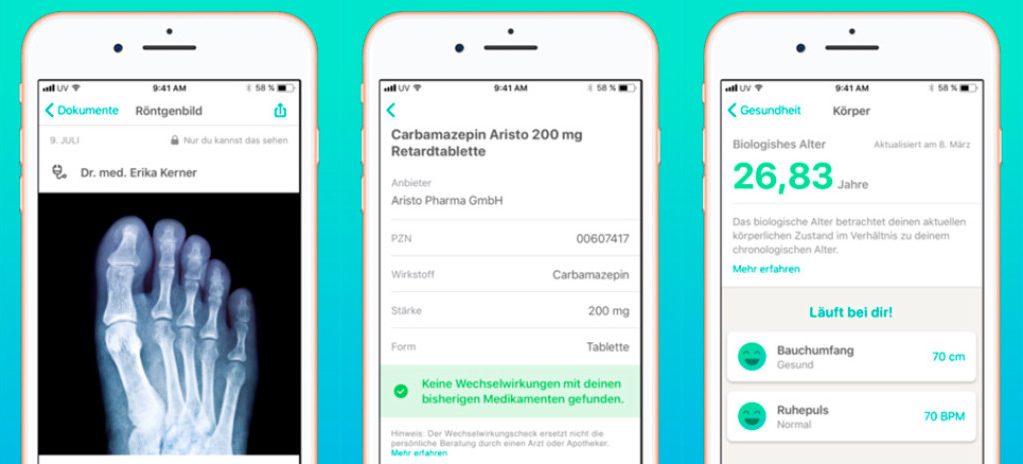
\includegraphics[width=\linewidth]{images/vivy2.png}
  \caption{Vivy App}
  \label{fig:vivy}
\end{figure}

Vivy\footnote{Vivy: \url{https://www.vivy.com/}. (Online; Last accesses November 18, 2019} is an application made by the German Vivy GmbH allowing users to manage their electronic health records. The security aspects of the app are reviewed by the Secure Systems Engineering department of the Fraunhofer AISEC in a whitepaper\cite{vivywhitepaper}.
\newline
Vivy follows the recommendations of the German Federal Office for Information Security (BSI) by complying to standards such as the BSI 200-1 and BSI 200-2. Vivy uses cryptographic protocols and cipher suites recommended by the BSI in their technical guidelines BSI TR-02102-1 and BSI TR-02102-2.
\newline
Below are some of their implemented security features that are of interest regarding this thesis:
    \paragraph{Two-factor Authentication} Vivy uses two-factor authentication for all its users. Beside the user made password the user’s smart phone is linked to his account.
    \paragraph{Data Encryption} All data saved on Vivy servers are encrypted with a user specific key, meaning that only the user can access the data using their private key. Vivy uses a hybrid encryption scheme, encrypting the data using a symmetric cryptographic technique, AES in GCM mode using a 256-bit key.  RSA using OAEP padding and 4096-bit keys is used to exchange the symmetric keys.
    \paragraph{Network Security} Vivy secures the communication and data exchange between its users by encrypting the data transferred and authenticating the communication partner. TLS 1.2 is used in the form of ELBSecurityPolicy-TLS-1-2-2017-01.


\section{CliniScale Project}
\label{cliniscale}
CliniScale is a project by the Databases and Information Systems Group\footnote{Databases and Information Systems: \url{https://www.mi.fu-berlin.de/en/inf/groups/ag-db/index.html}. (Online; last accessed:  November 18, 2019)} at Freie Universität Berlin with the goal to run clinical trials in the population. Combining web services with mobile applications enables clinical test centers to run scalable, user-friendly clinical trials in the population.\\
The main concept is to make clinical trials feasible in the population using mobile devices. The project provides solutions for the creation of clinical trials, proband selection procedures, executing the trial on a mobile device by selected probands and evaluation and presentation of the trial results.\\
Of interest for this thesis are the process, defined in section \ref{sysrequirements}, and the current implementation of the CliniScale back end and the Android mobile application, defined in section \ref{sysarchitecture}.


\section{Related Works}
\label{relatedwork}
\textit{Related Work} provides an overview on related scientific work, academic research and books covering the topics of
\textit{\nameref{subsection:riskass}}, \textit{\nameref{subsection:securecommunication}} and \textit{\nameref{subsection:privacyconcerns}}.

\subsection{Security Risk Assessment}
\label{subsection:riskass}


\cite{mora} by Jörn Eichler and Daniel Angermeier of the Fraunhofer AISEC presents the MoRA method to perform a security risk assessment. An in-depth explanation of this method can be found in the chapter \nameref{morachapter}. \cite{angermeier2016systematic} extends the original MoRA method on how to systematically identify security goals and threats. \cite{morasecgoals} further builds on the methodology by improving the identification, merging and validation of security goals.

\cite{cataloguerole} describes the role of threat and control catalogues in a security risk assessment. The actual and perceived qualitative and quantitative effect of using catalogues as part of a security risk assessment is researched. The quantitative analysis shows that non-security experts using catalogues reach results comparable to experts that are not using catalogues, while the perceived ease of use was slightly lower. It is also found out that security experts and non-experts have different expectations towards the catalogues. While experts are more interested in a common terminology and a checklist to validate that nothing was left out, non-experts are more interested in the ease of navigating through the catalogue, refusing larger and less specific catalogues.

In \cite{strideeval} the effectiveness of the Microsoft Threat Modeling Tool is evaluated by performing a course assignment on computer science graduates. The graduates performed two thread modeling tasks, first using a manual process and then using the threat modeling tool. Results show that the usage of the Microsoft Threat Modeling Tool improved the quality of the graduates work. The abstraction level of the defined model affects the amount of threats identified up to a point, were the number of generated threats is being limited.


\subsection{Secure Communication}
\label{subsection:securecommunication}


\cite{tlssysanalysis} presents an analysis of the TLS protocol and its application to data encryption. It shows how key encapsulation mechanisms can be extracted from the protocol and how the security of the entire protocol depends on the key encapsulation. This work suggests using CCA-secure implementations of the TLS protocol, as side channel attacks are possible on other variants.

In \cite{canetti2001analysis} the authors present a formalism for the analysis of key exchange protocols. Their findings are that any key exchange protocol can be paired with symmetric encryption and authentication functions in order to provide secure communication channels. Secure communication channels are a fundamental aspect of this thesis and Canetti and Krawczyk made fundamental groundwork in defining these and proving their security.

In \cite{sslandroid} the authors inspect the implementation of SSL/TLS protocols in android mobile applications by introducing MalloDroid, a tool to detect potential vulnerabilities against Man-In-The-Middle (MITM) attacks. 13500 popular applications have been investigated and 1074 revealed to be potentially vulnerable to MITM attacks. As a consequence, measurements categorized in three categories, OS solutions, App market solutions and Standalone solutions, are presented. The OS solutions are of interest. They recommend certificate pinning, usage of HTTPS in every connection, improved permission policies and visual security feedback.

\cite{cooijmans2014analysis} describes various ways of storing secret keys in a secure way on Android, analyzing both software and hardware solutions. A critical part of successfully implementing cryptography is to ensure a secure way to store the needed secret keys. The authors work describes different solutions and discusses their advantages, making it a good source for this thesis to base its design decisions on. 


\subsection{Privacy in Healthcare}
\label{subsection:privacyconcerns}

In \cite{wilkowska2012privacy} the authors perform a study researching two aspects of using medical assistive technologies, security and privacy. There is a focus laid on the perceived importance of these aspects by users. Results show that, while healthy adults insist on the highest security and privacy standards, elderly and adults with ailing health attributes have a perceived lower importance towards security and privacy since they value fast and continuous help and monitoring higher. This shows that people, especially those in greater need, are ready to accept cuts into their security and privacy for medical assistance, something that the pharmacy industry or governments may want to exploit. From a security standpoint of view, it shows that it is of utmost importance to guarantee high level of security and privacy standards to everybody, especially those who are willing to give them up for medical assistance and risk being exploited.

In \cite{meingast2006security} the authors study the current technological advances in the health care sector and its impact on security and privacy. Additionally, existing methods to handle these issues are presented. Many issues regarding health data are discussed, such as data access and storage, and solutions to these problems are presented and are of interest for this thesis. Authentication and encryption are required to comply with the GDPR.

\cite{cios2019uniqueness} presents the authors research on medical data mining and possible security and privacy issues. Topics discussed involve privacy-conserving medical data mining and ownership of medical data, both interesting for this thesis. Data anonymization is found to be a key element in preserving privacy while still allowing researchers access to the medical data. Additionally, the "right to explanation" of the GDPR is found to be in conflict with deep learning algorithms and neural networks, as often the logic found by them are black boxes that lack transparency when it comes to understanding how they arrived at their decisions.


\cite{chin2012measuring} perform a study examining users attitude towards security and privacy for mobile devices and how it differs from the user’s usage of traditional devices such as laptops and PCs. The survey shows, that generally, users are more concerned about security and privacy when using their phones. A large number of the participants do not perform privacy critical tasks on their phones. When the participants were asked to rationally explain their decisions, the main problems regarding security on a mobile devices can be traced back to lack of trust into communication technologies, such as Wi-Fi or 3G, mobile devices lack of anti-virus protection, lack of knowledge about mobile devices and the easiness to lose a mobile phone. Participants that were more concerned about security and privacy on laptops and PCs noted that they do not perform privacy critical tasks, such as banking or entering their social security number, on their mobile phone at all. Understanding the user’s motives and needs is an important factor in designing a privacy critical application. Complying and using international accepted standards may help improve the users trust into an application, making it viable to a larger audience. The authors present recommendations on how to improve user’s confidence towards security and privacy of a mobile application.



